\documentclass[letterpaper,10pt]{article}

\usepackage{enumitem}
\usepackage{titling}
\usepackage{listings}
\usepackage{url}
\usepackage{hyperref}
\usepackage{setspace}
\usepackage{subfig}
\usepackage{sectsty}
\usepackage{pdfpages}
\usepackage{colortbl}
\usepackage{multirow}
\usepackage{multicol}
\usepackage{relsize}
\usepackage{amsmath}
\usepackage{wasysym}
\usepackage{fancyvrb}
\usepackage[yyyymmdd]{datetime}
\usepackage{amsmath,amssymb,amsthm,graphicx,xspace}
\usepackage[titlenotnumbered,noend,noline]{algorithm2e}
\usepackage[compact]{titlesec}
\usepackage{XCharter}
\usepackage[T1]{fontenc}
\usepackage[scaled]{beramono}
\usepackage[normalem]{ulem}
\usepackage{booktabs}
\usepackage{tikz}
\usetikzlibrary{arrows,automata,shapes,trees,matrix,chains,scopes,positioning,calc}
\tikzstyle{block} = [rectangle, draw, fill=blue!20,
text width=2.5em, text centered, rounded corners, minimum height=2em]
\tikzstyle{bw} = [rectangle, draw, fill=blue!20,
text width=4em, text centered, rounded corners, minimum height=2em]

\definecolor{namerow}{cmyk}{.40,.40,.40,.40}
\definecolor{namecol}{cmyk}{.40,.40,.40,.40}
\renewcommand{\dateseparator}{-}

\let\LaTeXtitle\title
\renewcommand{\title}[1]{\LaTeXtitle{\textsf{#1}}}

\lstset{basicstyle=\footnotesize\ttfamily,breaklines=true}

\newcommand{\handout}[5]{
	\noindent
	\begin{center}
		\framebox{
			\vbox{
				\hbox to 5.78in { {\bf SE 350: Operating Systems } \hfill #2 }
				\vspace{4mm}
				\hbox to 5.78in { {\Large \hfill #4  \hfill} }
				\vspace{2mm}
				\hbox to 5.78in { {\em #3 \hfill \today} }
			}
		}
	\end{center}
	\vspace*{4mm}
}

\newcommand{\lecture}[3]{\handout{#1}{#2}{#3}{Lecture#1}}
\newcommand{\tuple}[1]{\ensuremath{\left\langle #1 \right\rangle}\xspace}

\newcommand{\Rplus}{\protect\hspace{-.1em}\protect\raisebox{.35ex}{\smaller{\smaller\textbf{+}}}}
\newcommand{\Cpp}{\mbox{C\Rplus\Rplus}\xspace}


\addtolength{\oddsidemargin}{-1.000in}
\addtolength{\evensidemargin}{-0.500in}
\addtolength{\textwidth}{2.0in}
\addtolength{\topmargin}{-1.000in}
\addtolength{\textheight}{1.75in}
\addtolength{\parskip}{\baselineskip}
\setlength{\parindent}{0in}
\renewcommand{\baselinestretch}{1.5}
\newcommand{\term}{Winter 2023}
\newcommand{\termnumeric}{1231}

\singlespace


\begin{document}

\lecture{ 1 --- Introduction, Operating Systems, Security }{\term}{Jeff Zarnett}

\section*{About the Course}
We'll start by reviewing the highlights of the class syllabus. Please read it carefully (it is available in Learn under Content $\rightarrow$ Overview). It contains a lot of important information about the class including: the lecture topics, the grading scheme, contact information for the course staff, and university policies.

\section*{Introduction to Operating Systems}


\begin{quote}
\textit{Operating systems are those programs that interface the machine with the applications programs. The main function of these systems is to dynamically allocate the shared system resources to the executing programs.}

\textit{But the interface with adjacent levels continues to shift with
time. Functions that were originally part of the operating system have migrated to the hardware. On the other side, programmed functions extraneous to the problems being solved by the application programs are included in the operating system.
}
\end{quote}

\hfill - What Can Be Automated?: The Computer Science and Engineering Research Study, MIT Press, 1980

An operating system (often abbreviated OS) is a piece of software that sits between the hardware of a computer and the applications (programs) that run on that computer. The OS does many different things and often has many (occasionally-conflicting) goals. 

To use an analogy, you may wish to think of the operating system as the ``secretary'' of the computer.  It is a resource manager, and it allocates resources as necessary.  The most significant difference between a secretary and an operating system is that while a secretary can work in parallel with you, operating systems often work when programs are sleeping, and operating systems must put themselves to sleep to allow programs to execute. It is responsible for seeing to it that other programs can operate efficiently, providing an environment for other programs, and collecting and reporting data about what is and has been happening.

\begin{center}
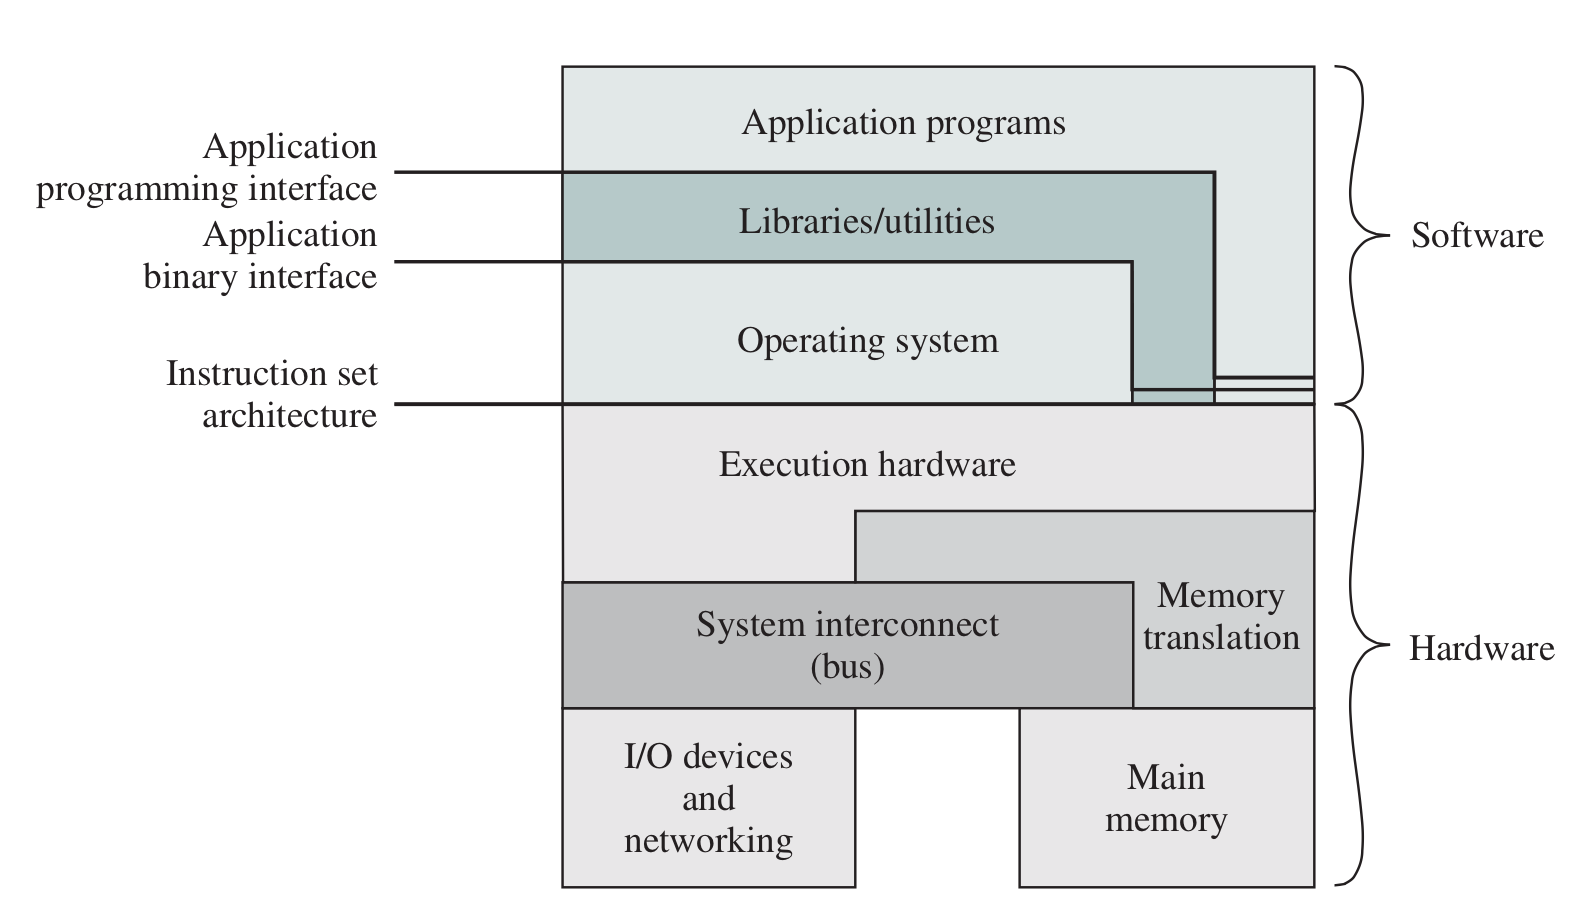
\includegraphics[width=0.73\textwidth]{images/os-sw-hw.png}\\
Structural diagram of a modern computer~\cite{osi}.
\end{center}

An operating system is also responsible for resource allocation. In the real world, the resources we have to work with, such as CPU time or memory space, are limited. The OS decides how to allocate these resources, keeps track of who currently owns what, and, in the event of conflicting requests, determines who gets the resource.

The OS usually enables useful programs like Photoshop or Microsoft Word to run. Any computer has various pieces of hardware, such as the CPU, memory, input/output devices (such as monitors, keyboards, modems). The OS is responsible for abstracting away the details of this, so that the authors of programs do not have to worry about the specifics of the hardware. Imagine how painful it would be to write even a simple program, like the Hello World example, if we had to write our program differently for every combination of hardware.

In most cases there will be multiple programs running on the computer. This implies the sharing of various resources. When this is the case, there is the potential for conflicts to arise. An operating system creates and enforces rules to make sure all the programs get along and play fairly. Of course, not all interaction between programs is competitive; sometimes they want to co-operate, and the OS helps them do that, too.

Another goal may be to use the computer hardware efficiently. This is not usually an issue with personal laptops, but imagine a supercomputer. A supercomputer used to do extremely complex computations is expensive to build and maintain. Any moment when the supercomputer is not doing useful work is a costly waste, so an operating system for such a computer would try to maximize CPU usage. There is, after all, only so much CPU time in supercomputers and there are many programs eager to run (weather simulations, particle physics simulations...).

Operating systems tend to be large and do a lot of things. We expect now that an OS comes with a web browser, an e-mail client, some method for editing text, et cetera. These things, while important and useful, are not what we are going to focus on. The part of the operating system that we will study is what we call the \textit{Kernel} - it is the ``core''; the portion of the OS that is always present in main memory and the central part that makes it all work.

Operating systems will evolve over time. There will be new hardware released, new types of hardware, new services added, and bug fixes. Evolution is constrained by a need to maintain compatibility for programs. If the user upgrades his or her desktop OS and a program breaks, even if it's the program author's fault, the user blames the OS vendor. If you look at Microsoft Windows, you can see their strict devotion to not breaking binary compatibility (at least, as much as they reasonably can). Linus Torvalds, yes, the person Linux is named after, gets unreasonably angry with people if they submit a kernel change that might break user-space programs. 

As we proceed we will focus on UNIX-like systems with some mention of Microsoft Windows where appropriate. This is for practical reasons: there is only so much time and UNIX-like systems represent a very large percentage of the operating systems out there including Linux, Mac OS X, Android, and more.

\section*{Security Now}
When I taught a previous operating systems course, ECE 254, here we spent some time talking about the history of operating systems and how we got to the modern generations of them. While some understanding of the history of a thing might be helpful in explaining some design decisions, the discussion was too vague and high-level to be useful. Nice trivia, maybe. So instead we are going to talk about security.

In a lot of textbooks, security is left to the end. This strikes me as being a problem: security is something you want to bake into your design and something you want to have in your mind constantly. It doesn't work to try to bolt it on afterwards. As we go through the topics of the course, we aren't going to stop at every opportunity to consider the security implications or risks of each implementation or decision... but it would still be a good idea to think about security in each situation.

An operating system is designed to support multiple users concurrently, each of whom are likely running multiple programs concurrently too. There are also the operating system's processes itself, which are not really under the user's control either. Even if you are the only user on your system, the operating system will enforce certain rules so that malicious programs (or malicious websites) can't steal your personal data or sabotage the system. 

Typically, OS designers create some policies and also policy tools. Some policies are just a part of the operating system and cannot be changed -- e.g., a file must have the ``execute'' permission to run. Others are configurable by system administrators -- e.g., may non-administrator users install new programs on the system? Security policies do have some tradeoff with usability, in that it can be frustrating for users who are denied some operation and must instead ask administrators to do it for them. But you also can't be too lax about this, because you most certainly do NOT want to find your company's name on TV having to report a data breach in which user personal data was stolen.

OS designers must see to it that the security policies (whether configured or not) are enforced consistently. This helps to ensure that sensitive data is protected, not corrupted, and only accessed by those who should have access. Operating systems that do not provide proper protection and security will inevitably be exploited by malicious users and it will cease to be used. 

\paragraph{Protection vs. Security} It's important to draw a quick distinction between \textit{protection} and \textit{security} as in~\cite{osc}. Protection is about controlling the access of programs and processes 


\bibliographystyle{alphaurl}
\bibliography{350}


\end{document}